\section{Alimentation}

Le schéma électronique de l'alimentation de la figure \ref{fig:alim} possède un fusible d'entrée.
Sa fonction est de protéger les diverses composantes du robot.
Chacune des composantes est munie d'un interrupteur.
Des connecteurs MTA-156 sont utilisés pour faire le raccord entre le PCB d'alimentation et les dévolteurs.
En ce qui concerne le dévolteur de l'ordinateur embarqué, il est directement fixé au PCB d'alimentation.
Chacun des interrupteurs supporte un courant de 3A.
Des fils AWG 18 sont présents pour faire les différents raccords, ce qui est amplement suffisant pour l'ensemble des courants possibles et
ils permettent de minimiser la résistance. Un indicateur au LED est toujours pratique pour visualiser la présence de l'alimentation sur le PCB
provenant de la batterie Lipo. Des traces de 3mm sont utilisées pour limiter la présence de résistance inutile
et un plan de masse au-dessus du PCB a été mis en place.

\paragraph{}
Le shield de l'Arduino représenté à la figure \ref{fig:shield} permet un raccord facilité avec le pont H et les 4 moteurs roues.
Le PCB élimine un grand nombre de fils et il relie l'Arduino avec le drive de la bobine ainsi que pour le décodage du code Manchester.
Un plan de masse est présent sur l'ensemble du dessus du PCB.


\begin{landscape}
  \begin{figure}[ht]
    \centering
    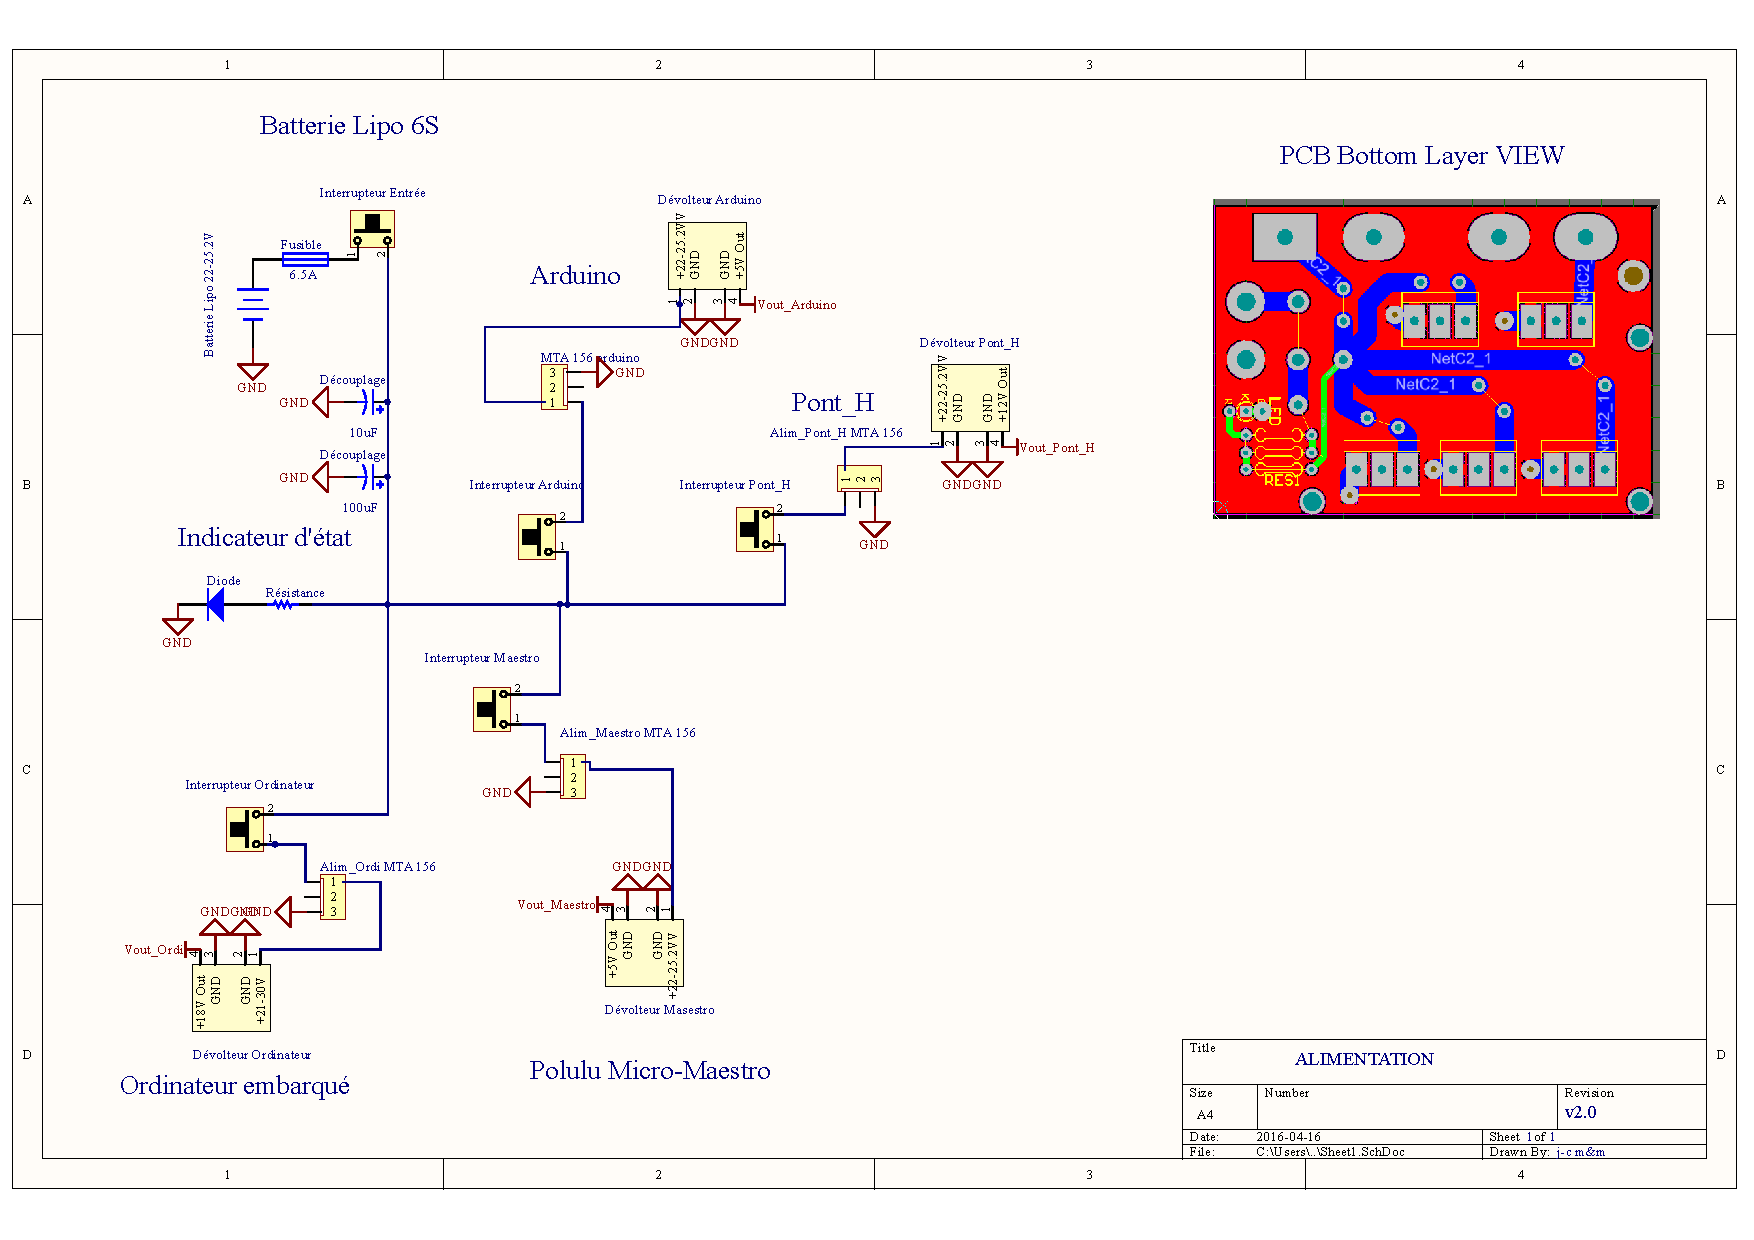
\includegraphics[scale=0.6]{resources/alim.pdf}
    \caption{Schéma électronique de l'alimentation}
    \label{fig:alim}
  \end{figure}

  \begin{figure}[ht]
    \centering
    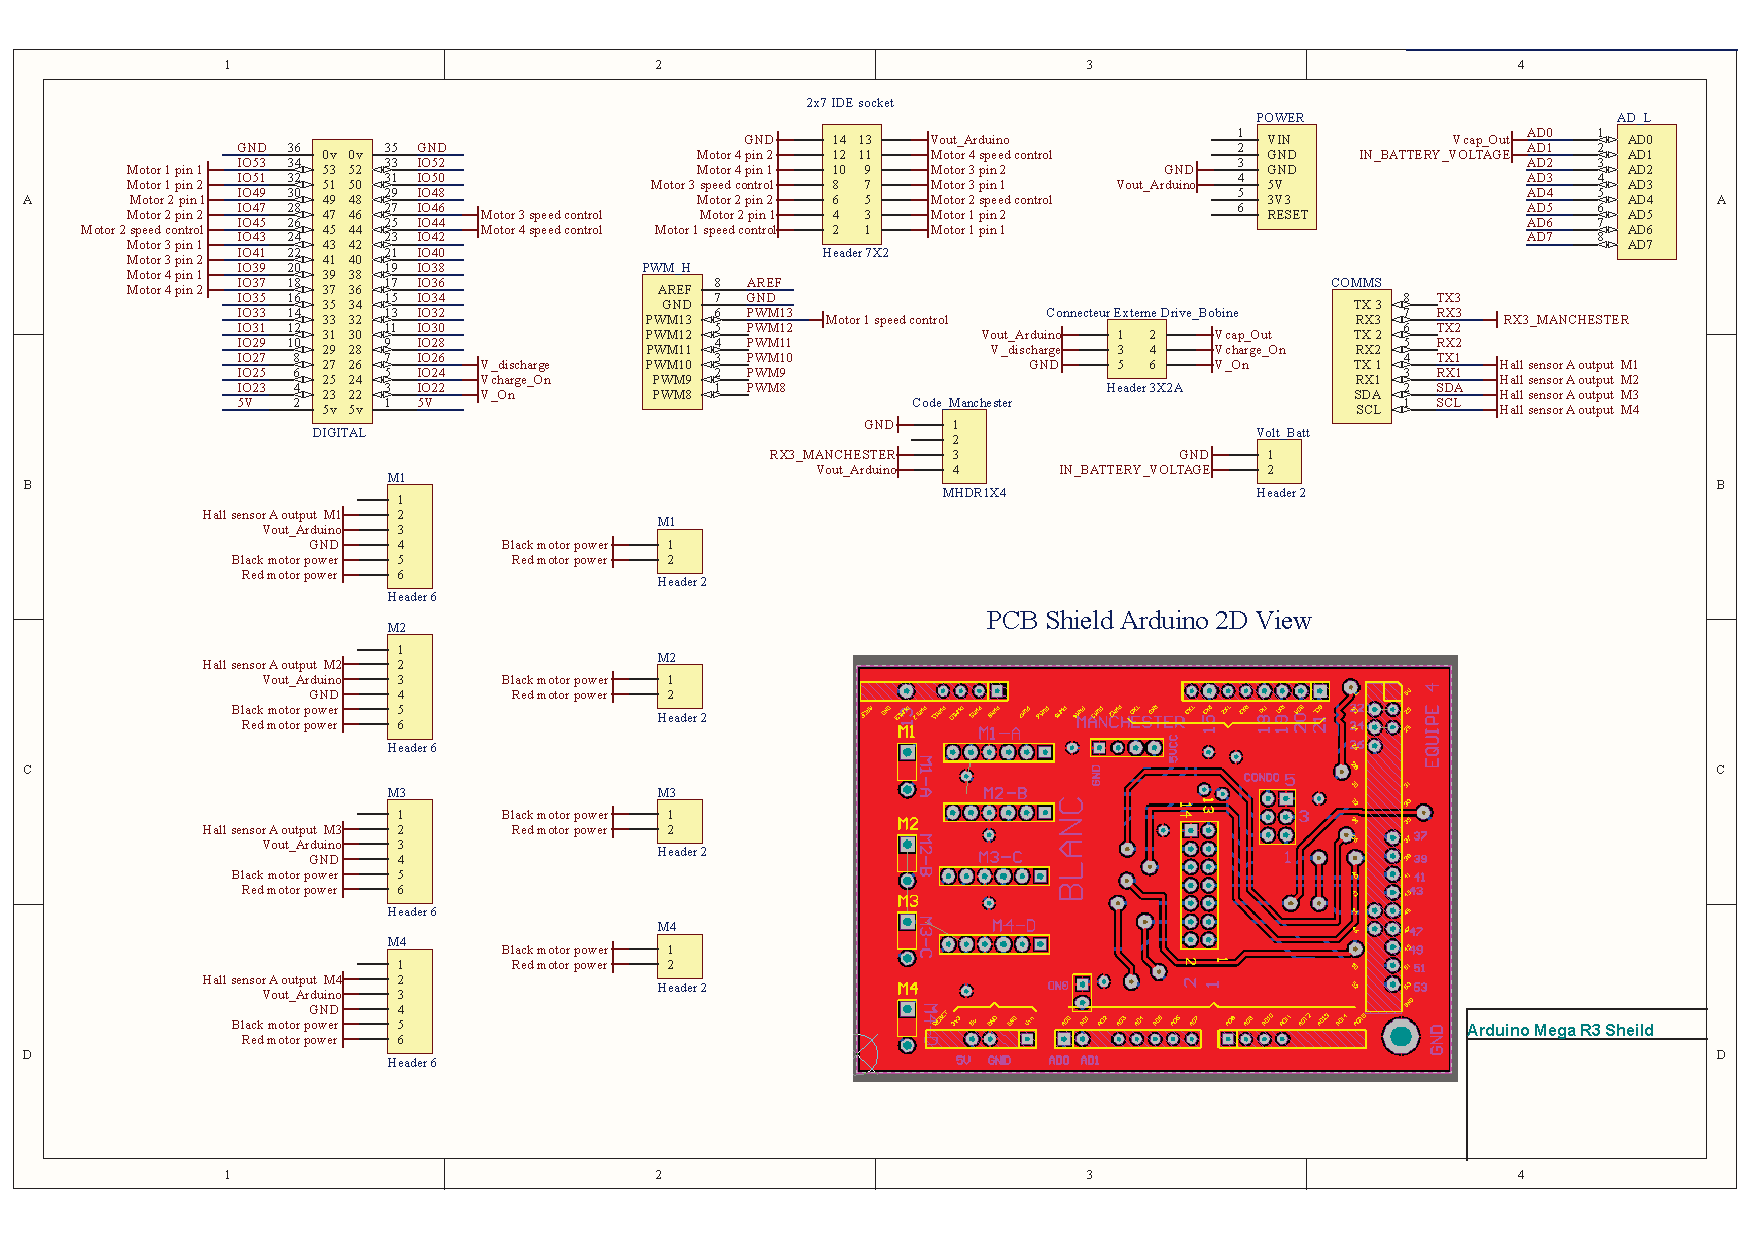
\includegraphics[scale=0.6]{resources/shield.pdf}
    \caption{Schéma électronique du shield de l'arduino}
    \label{fig:shield}
  \end{figure}
\end{landscape}
